\begin{surferIntroPage}{World Record Surfaces}{record_chmutovoktic}{World Record Surfaces}
    A surface is called \emph{non-singular} or \emph{smooth} if it does not have any apex (such points are called \emph{singularities}). Examples of smooth surfaces are a sphere or a torus, see the first 2
    pictures below.  
    This is almost sure the case when choosing a random surface. 
 \begin{center}
      \vspace{-0.2cm}
      \begin{tabular}{@{}c@{}c@{}c@{\quad}c@{}c@{}c@{}c@{}}
        \begin{tabular}{@{}c@{}}
          smooth:
        \end{tabular}
        &
        \begin{tabular}{@{}c@{}}
          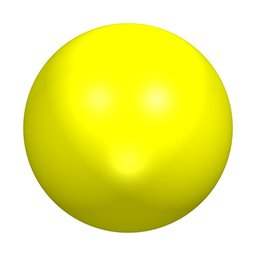
\includegraphics[width=1.1cm]{./../../common/images/kugel}
        \end{tabular}
        &
        \begin{tabular}{@{}c@{}}
          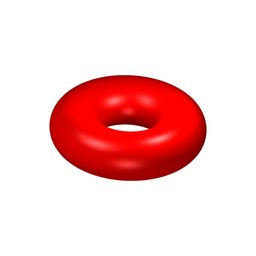
\includegraphics[width=1.1cm]{./../../common/images/torus}
        \end{tabular}
        &
        \begin{tabular}{@{}c@{}}
          many\\
          singularities:
        \end{tabular}
        &
        \begin{tabular}{c@{}@{}}
          
\includegraphics[width=1.1cm]{./../../common/images/kummer}
        \end{tabular}
        &
        \begin{tabular}{c@{}@{}}
          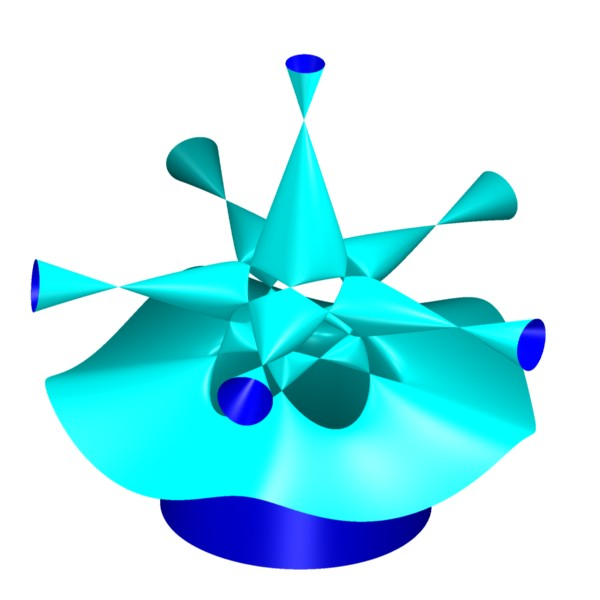
\includegraphics[width=1.1cm]{./../../common/images/togliatti}
        \end{tabular}
        &
        \begin{tabular}{c@{}@{}}
          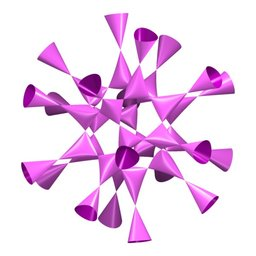
\includegraphics[width=1.1cm]{./../../common/images/barth_sextic}
        \end{tabular}
      \end{tabular}
    \end{center}
    \vspace{-0.2cm}
    Thus it is very special when a surface exhibits singularities. They are the most interesting points of a surface. The surfaces in the SURFER programme are defined by polynomials. The highest power of a polynomial is called its degree $d$. Mathematicians ask how many singularities  a surface of a certain degree may have.
    We will denote this number by $\mu(d)$.

 It turns out that this number $\mu(d)$ is very difficult to compute.
    Since the $19$th century, $\mu(d)$ is known for $d=1,2,3,4$, but for $d=5$
    this number was only identified in 1980, and for $d=6$ in 1996.
    For $d\ge 7$, $\mu(d)$ is still unknown.
  
    So, every new world record for a $\mu(d)$ is an important partial result. It seems to take a lot more time to completely solve this problem for arbitrary $d$.\\  A few known results:
    
   \begin{center}
      \begin{tabular}{r|cccccccc|c}
        $d$ & $1$ & $2$ & $3$ & $4$ & $5$ & $6$ & $7$ & $8$ & $d$\\
        \hline
        \hline
        \rule{0pt}{1.2em}$\mu(d)\ge$ & $0$ & $1$ & $4$ & $16$ & $31$ & $65$ &
        $99$ & $168$ & 
        $\approx \frac{5}{12}d^3$\\[0.3em]
        \hline
        \rule{0pt}{1.2em}$\mu(d)\le$ & $0$ & $1$ & $4$ & $16$ & $31$ & $65$ &
        $104$ & $174$ & $\approx \frac{4}{9}d^3$
      \end{tabular}
    \end{center}
\end{surferIntroPage}
